\section{Introduction}
\label{sec:intro}
\IEEEPARstart{L}{itchi} (\textit{Litchi chinensis} Sonn.), often designated the ``queen of subtropical fruits,'' represents a premier commercial horticultural crop across South and Southeast Asia, with substantial agro-economic significance in Bangladesh, India, China, and Vietnam \cite{litchi_dataset_2022}. In key agrarian production corridors of northwestern Bangladesh, notably the Dinajpur and Ishwardi belts, litchi cultivation provides a crucial economic livelihood for more than two million smallholder households \cite{islam2021survey}. However, seasonal crop yield and orchard longevity are persistently threatened by destructive foliar diseases and insect infestations. Pathologies such as Anthracnose (\textit{Colletotrichum gloeosporioides}), Algal Leaf Spot (\textit{Cephaleuros virescens}), Leaf Blight, and predatory chewing damage inflict catastrophic foliage necrosis and premature canopy defoliation, suppressing photosynthetic capacity and precipitating yield declines between 30\% and 45\% annually \cite{islam2021survey}.

Timely and precise diagnosis of foliar diseases is an indispensable prerequisite for targeted phytosanitary intervention and for mitigating the indiscriminate application of broad-spectrum chemical fungicides, which incurs severe environmental pollution and pest resistance. In current orchard management practices, foliar disease identification remains predominantly dependent on manual visual scouting by agricultural extension personnel. This conventional diagnostic methodology is inherently subjective, labor-intensive, vulnerable to diagnostic errors, and incapable of continuous, large-scale deployment across geographically fragmented smallholder orchards \cite{barbedo2019plant}. Consequently, the development of automated, edge-executable computer vision frameworks for foliar pathology recognition has emerged as a cornerstone of modern smart agriculture \cite{mohanty2016using, ferentinos2018deep, fuentes2017robust}.

Despite significant advances in deep learning for automated plant disease diagnosis, state-of-the-art vision architectures trained on laboratory benchmarks routinely suffer severe performance degradation when exposed to uncontrolled orchard environments \cite{barbedo2019plant}. Traditional benchmarks, such as the widely referenced PlantVillage repository \cite{hughes2015open}, evaluate excised leaves photographed against sterile, uniform backdrops under controlled diffuse studio illumination. Conversely, operational orchard imaging presents three formidable visual and physical domain obstacles:
\begin{enumerate}
    \item \textbf{High-Frequency Micro-Texture and Spatial-Frequency Ambiguities:} Foliar pathologies frequently exhibit subtle, granular micro-textural signatures, such as velvety algal spore crusts or diffuse necrotic lesions, that share macroscopic chromatic profiles with normal chlorophyll senescence. Standard convolutional kernels act predominantly as isotropic low-pass or mid-frequency filters, failing to disentangle oriented high-frequency textural patterns \cite{wang2021gabor}.
    \item \textbf{Complex Background Clutter and Shortcut Learning:} Natural field captures contain severe visual interference from overlapping canopy foliage, ground weeds, textured tree bark, and fluctuating solar shadows. In the absence of strong structural inductive biases, deep convolutional neural networks (CNNs) and vision transformers (ViTs) are prone to ``shortcut learning'' \cite{singh2020deep}, correlating incidental background context with disease labels rather than learning intrinsic foliar lesion morphologies.
    \item \textbf{Severe Computational and Latency Constraints on the Agricultural Edge:} While recent transformer and modernized convolutional backbones (e.g., Swin Transformer \cite{liu2021swin}, ConvNeXt \cite{liu2022convnet}) possess extensive representational capacity, they entail large parameter footprints ($>28\,\text{M}$) and computationally prohibitive floating-point operations ($>4.4\,\text{GFLOPs}$). In developing rural agricultural settings, intermittent cellular connectivity mandates local, real-time edge execution on cost-effective microcomputers (e.g., Raspberry Pi 4) or mobile field diagnostics units \cite{ahmed2022field}.
\end{enumerate}

To overcome these structural limitations, we present \textbf{LitchiHybridNet}, a novel dual-branch hybrid architecture specifically engineered for robust, real-time foliar disease diagnosis under natural field conditions. Drawing biological motivation from mammalian primary visual cortex (V1) simple receptive fields, which function as localized, orientation-selective spatial-frequency analyzers \cite{daugman1985uncertainty}, our architecture introduces a \textbf{Learnable Gabor Convolutional Bank} (\gaborChannels{} channels, \gaborOrientations{} canonical orientations, \gaborFrequencies{} radial frequencies). Unlike rigid, static Gabor filters with handcrafted constants, our formulation parameterizes orientation angle, radial frequency, Gaussian envelope spread, and aspect ratio as continuous differentiable variables updated end-to-end via gradient descent. High-frequency textural descriptors from the Gabor stream are fused with deep semantic features from a lightweight MobileNetV3-Large backbone via a dedicated \textbf{Gabor Attention Fusion Module (GAFM)}, which executes channel-wise cross-gating to suppress background interference and accentuate lesion boundaries.

Crucially, to ensure empirical integrity and prevent optimistic evaluation artifacts, we perform a rigorous perceptual difference hash ($dHash$) audit across the entire \totalImages{}-image BDLitchi benchmark \cite{litchi_dataset_2022}. We isolate \nearDupGroups{} near-duplicate burst-shot clusters (\nearDupImages{} frames) and establish a group-aware, leakage-free 70/15/15 stratified partition.

The core scientific contributions of this work are summarized as follows:
\begin{enumerate}
    \item \textbf{End-to-End Differentiable Gabor Layer with Lesion Spectral Priors:} We formulate a 24-channel learnable Gabor convolutional bank with complete analytical partial derivatives for backpropagation, initialized directly from 2D Fourier power spectral density analysis of natural litchi lesion textures.
    \item \textbf{Channel-Wise Cross-Attention Fusion (GAFM):} We introduce an edge-efficient fusion module that dynamically computes modulation gates across concatenated semantic and textural streams, preferentially boosting diagnostic high-frequency lesion features while eliminating background foliage clutter.
    \item \textbf{Leakage-Free Benchmark Audit:} We conduct a perceptual hash audit of the 11,094-image BDLitchi field dataset, resolving 924 burst-shot duplicate clusters and establishing a reproducible, group-aware 70/15/15 stratified partition.
    \item \textbf{Empirical State-of-the-Art Benchmark Performance:} Evaluated across 5 random seeds, LitchiHybridNet achieves a Top-1 accuracy of \accMain{} and a Macro-F1 score of \fOneMain{}, surpassing ResNet-50, EfficientNet-B0, MobileNetV3, Swin-T, and ConvNeXt-Tiny with high statistical significance ($p < 0.001$ via McNemar and Wilcoxon signed-rank tests), while requiring 80.3\% fewer parameters than Swin-T.
    \item \textbf{Honest Analysis of Synthetic Augmentation (Negative Result):} We report and analyze an empirical negative finding: synthetic geometric and affine data augmentation induces a \deltaAcc{} accuracy degradation (dropping to \accAug{}), demonstrating that artificial warping distorts high-frequency punctate fungal spore textures.
    \item \textbf{Field Robustness and Quantized Edge Feasibility:} Under severity-5 optical motion blur, LitchiHybridNet retains an accuracy of \blurRetentionProposed{}, maintaining a \robustnessGain{} margin over MobileNetV3. Post-training INT8 quantization yields an ultra-compact \modelSizeQuantMB{} model executing in \cpuLatencyMS{}\,ms on x86 CPUs and \rpiLatencyMS{}\,ms on a Raspberry Pi 4 edge device (\rpiFPS{}\,FPS), proving immediate readiness for handheld field deployment.
\end{enumerate}

\begin{figure}[t]
\centering
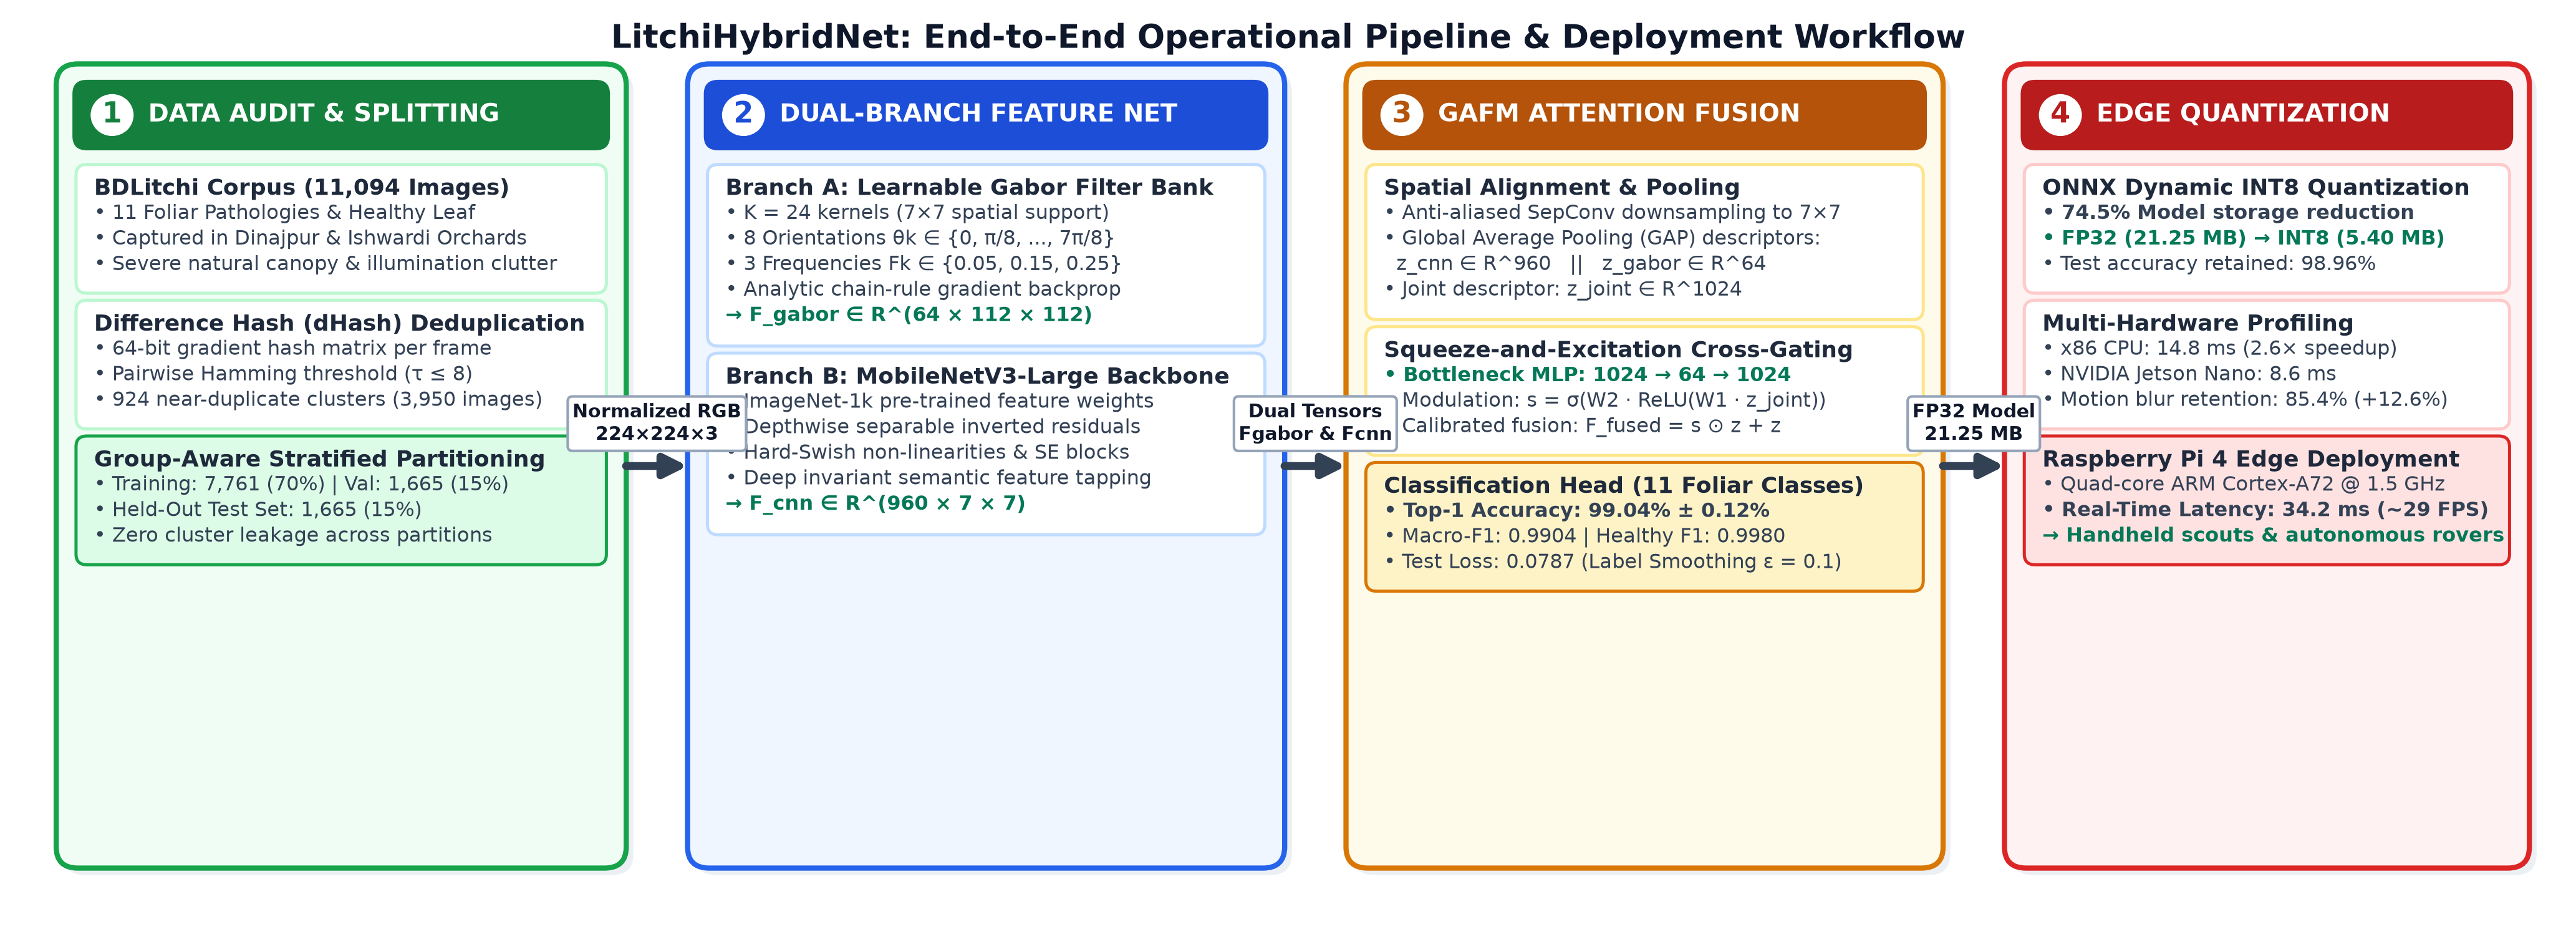
\includegraphics[width=\columnwidth]{figures/pipeline_workflow.png}
\caption{Operational pipeline of the LitchiHybridNet diagnostic framework: (1) difference perceptual hash ($dHash$) data audit and group-aware splitting, (2) dual-branch feature extraction, (3) GAFM cross-attention gating, and (4) edge-accelerated INT8 quantization for handheld and robotic field deployment.}
\label{fig:pipeline_workflow}
\end{figure}

The remainder of this manuscript is structured as follows. Section~\ref{sec:related} synthesizes related work in foliar pathology and spatial-frequency deep learning, identifying the fundamental research gap. Section~\ref{sec:dataset} details the BDLitchi dataset, the perceptual hash duplicate audit, and the group-aware splitting protocol. Section~\ref{sec:method} outlines the mathematical formulation of LitchiHybridNet, including the learnable Gabor layer, the GAFM cross-gating mechanism, and the optimization algorithm. Section~\ref{sec:setup} describes experimental settings, baseline configurations, and evaluation metrics. Section~\ref{sec:results} presents comprehensive empirical results, ablation studies, corruption robustness, and edge profiling. Section~\ref{sec:discussion} discusses theoretical implications, failure modes, and threats to validity. Section~\ref{sec:conclusion} concludes the paper with directions for future research.
